%!TEX root = P231_notes.tex

\section{Kramers--Kronig [optional]}
% \lecdate{lec~12}
% 2017 Lec 17ish

\subsection{Cauchy Principal Value}
% See Cohen, "Complex Analysis with Applications to Science and Engineering"
% p. 139

We have seen that the pole structure of an integrand has physical significance. When solving for the harmonic oscillator Green's function, we saw that we had to \emph{change} the nature of the harmonic oscillator differential operator in order to derive the \emph{retarded} (causal) Green's function rather than the \emph{advanced} (acausal) Green's function. In that case, we found a real integral with a pole along the integration axis and decided that the integrand itself was the problem.

What happens if \emph{we don't want to change the integrand?} For example, most physicists wouldn't object too much that the integral
\begin{align}
	\int_{-1}^4 dx\, \frac{1}{x-1}
\end{align}
should have a well defined value even though there is a simple pole at $x=1$. In fact, with a bit of thought (try sketching the integrand on a graph), one may argue that
\begin{align}
	\int_{-1}^4 dx\, \frac{1}{x-1}
	= 
	\int_{3}^4 dx\, \frac{1}{x-1}
\end{align}
because the integrand is antisymmetric about the pole. Sure, the integrand is undefined at $x=1$, but every contribution just to the right of the pole, say $x=1+\varepsilon$ is exactly canceled by a contribution just to the left of the pole, $x=1-\varepsilon$. This is purely \emph{real} calculus.

The \textbf{Cauchy principal value} of a real integral with a pole along the integration contour (the real axis) formalizes this idea. Suppose $f(x)$ is well behaved (analytic) along the real axis. For an integrand $f(x)/(x-x_0)$, the Cauchy principal value is defined to be
\begin{align}
	\mathcal P \int_{-\infty}^\infty dx\, \frac{f(x)}{x-x_0}
	= 
	\lim_{\varepsilon\to 0}
	\left[
	\int_{-\infty}^{x_0-\varepsilon} dx\, \frac{f(x)}{x-x_0}
	+\int_{x_0+\varepsilon}^\infty dx\, \frac{f(x)}{x-x_0}
	\right] \ .
\end{align}
In other words, you simply integrate everywhere except the pole along the real axis. Formally we cannot say anything about the integrand at $x=x_0$, but perhaps part of you secretly thinks this is not a big deal since the $\varepsilon\to 0$ limit is well behaved. Again, thus far we are only doing real calculus.

\flip{Include picture}

\paragraph{Relation to a contour.} We can now connect to complex analysis. Suppose $f(x)$ is well behaved enough that we can imagine integrating $f(z)/(z-x_0)$ along a closed contour with the integral along the ``arc at infinity'' (either in the upper or lower half plane) going to zero. Then we can write the following:
\begin{align}
	\int_{C(\gamma_\pm)} dz \; \frac{f(z)}{(z-x_0)} &= 
	\int_{-\infty}^{x_0-\varepsilon} dx\, \frac{f(x)}{x-x_0}
	+
	\int_{x_0+\varepsilon}^\infty dx\, \frac{f(x)}{x-x_0}
	+
	\int_{\gamma_\pm} dz \; \frac{f(z)}{(z-x_0)}
	+
	\int_{\text{arc}} dz \; \frac{f(z)}{(z-x_0)} \ .
	\label{eq:cauchy:contour}
\end{align}
By assumption, the last term goes to zero. The first two terms are the Cauchy principal value when $\varepsilon\to 0$. The third term along contour $\gamma$ is a small semicircle of radius $\varepsilon$ that connects the two contours of the Cauchy principal value. It's a little semicircle that either goes just above ($\gamma_+$) or just below ($\gamma_-$) the real axis. Of course, you already realize the important point: the contour $C$ \emph{depends} on the choice of $\gamma_\pm$. This determines whether or not the point $z=x_0$ is inside or outside the contour.

\paragraph{Residue Theorem.} Let us assume that the integrand $f(z)/(z-x_0)$ is such that one can close the integral along the upper-half plane.\footnote{The argument is completely analogous if it were to be closed along the lower-half plane} This means that $f(z)/(z-x_0) \to 0$ fast enough as the radius of the semicircle goes to $R\to \infty$.\footnote{Remind yourself why `fast enough' is $1/R^2$ or faster.} Now the residue theorem tells us that
\begin{align}
	\int_{C(\gamma_\pm)} dz \; \frac{f(z)}{(z-x_0)} &= 2\pi i \sum_j \text{Res}_F(z_j)
	&
	F(z) = \frac{f(z)}{(z-x_0)} \ ,
\end{align}
where $j$ runs over the poles enclosed in $C(\gamma_\pm)$. When we take $\gamma_+$, this means that the poles do not include $x_0$. When we take $\gamma_-$, the poles do include $x_0$. The residue at $x_0$ is
\begin{align}
 	\text{Res}_F(x_0) &= f(x_0) \ .
\end{align}
In general, we expect $f(z)$ to have its own poles off the real axis; if any of those poles simple and are enclosed then they contribute to the sum. Just remember that if $z_j$ is a simple pole of $f(z)$, then the relevant residue is $(z_j-x_0)^{-1}\text{Res}_f(z_j)$.\footnote{Take the time to remind yourself why this is true if it is not obvious.}

\paragraph{Little semi-circles.}
The next step is to identify what the $\gamma_\pm$ integrals give. We may use the parameterization $z=x_0+\varepsilon e^{i\theta}$ to write
\begin{align}
	\int_{\gamma_+} dz \; \frac{f(z)}{(z-x_0)}
	&=
	\int_{\pi}^0 i\varepsilon e^{i\theta} d\theta \frac{f\left(x_0+\varepsilon e^{i\theta}\right)}{\varepsilon e^{i\theta}}
	=
	-i \pi f(x_0) \ .
\end{align}
We went ahead and took the $\varepsilon\to 0$ limit, implicitly using the analyticity of $f(z)$ at $z=x_0$. Similarly, if we used $\gamma_-$ as part of our contour,
\begin{align}
	\int_{\gamma_-} dz \; \frac{f(z)}{(z-x_0)}
	&=
	\int_{\pi}^{2\pi} i\varepsilon e^{i\theta} d\theta \frac{f\left(x_0+\varepsilon e^{i\theta}\right)}{\varepsilon e^{i\theta}}
	=
	+i \pi f(x_0) \ .
\end{align}

\paragraph{Putting it all together.}
We may then write \eqref{eq:cauchy:contour} as
\begin{align}
	\int_{C(\gamma_\pm)} dz \; \frac{f(z)}{(z-x_0)} &= 
	\mathcal P
	\int_{-\infty}^\infty dx\, \frac{f(x)}{x-x_0}
	+
	\int_{\gamma_\pm} dz \; \frac{f(z)}{(z-x_0)}
\end{align}
so that
\begin{align}
	\mathcal P
	\int_{-\infty}^\infty dx\, \frac{f(x)}{x-x_0}
	&=
	2\pi i \sum_j \left.\text{Res}_F(z_j)\right|_{C_\pm}
	\pm i \pi f(x_0) \ ,
	\label{eq:cauchy:principal:wrt:residues}
\end{align}
where we remind ourselves that the choice of contour ($\pm$) determines both the sign of the $\mp i \pi f(x_0)$ term \emph{and} whether or not the pole $z=x_0$ is enclosed by $C_\pm$. 
\begin{exercise}
Confirm that the right-hand side of \eqref{eq:cauchy:principal:wrt:residues} is independent of whether one closes the contour with $\gamma_+$ or $\gamma_-$.
\end{exercise}

\paragraph{Cauchy principal value and the $i\varepsilon$ notation.} %see Cohen.

Let us continue to assume that the contour $C$ is closed by an arc in the upper-half plane.\footnote{Recall that this amounts to an assumption about the convergence of $F(z)$ as $z\to Re^{i\theta}$ for large $R$ and $0 < \theta < \pi$.}
It is clear that closing the contour $C(\gamma_+)$ with $\gamma_+$ corresponds to excluding the pole at $z=x_0$ from the sum of residues. This means it is equivalent to a contour with the uninterrupted entire real axis $C_0$ for a modified integrand where the pole has been pushed downward:
\begin{align}
	\int_{C(\gamma_+)} dz \, \frac{f(z)}{z-x_0}
	=
	\lim_{\varepsilon\to 0}
	\int_{C_0} dz \, \frac{f(z)}{z-(x_0-i\varepsilon)} \ .
\end{align}
Similarly, for the contour $C(\gamma_-)$ with $\gamma_-$, the integral is equivalent to the contour that includes the uninterrupted real axis $C_0$ for a modified integrand where the pole is pushed upward into the contour:
\begin{align}
	\int_{C(\gamma_-)} dz \, \frac{f(z)}{z-x_0}
	=
	\lim_{\varepsilon\to 0}
	\int_{C_0} dz \, \frac{f(z)}{z-(x_0+i\varepsilon)} \ .
\end{align}
This gives a way to write \eqref{eq:cauchy:principal:wrt:residues} independently of the $\gamma_\pm$:
\begin{align}
	\mathcal P
	\int_{-\infty}^\infty dx\, \frac{f(x)}{x-x_0}
	&=
	% 2\pi i \sum_j \left.\text{Res}_F(z_j)\right|_{C_\pm}
	\lim_{\varepsilon\to 0}
	\int_{C_0} dz \, \frac{f(z)}{z-(x_0\mp i\varepsilon)} \ 
	% \mp i \pi \int dx\; f(x) \delta(x-x_0) \ .
	\pm i \pi f(x_0) \ .
\end{align}
Recalling that the contour integral over $C_0$ is really just the integral along the real line plus a vanishing integral over the arc, we may write the right-hand side as a real integral:
\begin{align}
	\mathcal P
	\int_{-\infty}^\infty dx\, \frac{f(x)}{x-x_0}
	&=
	% 2\pi i \sum_j \left.\text{Res}_F(z_j)\right|_{C_\pm}
	\lim_{\varepsilon\to 0}
	\int_{-\infty}^\infty dx\; f(x)\left[
		\frac{1}{x-(x_0\mp i\varepsilon)} \ 
		\pm i \pi   \delta(x-x_0) 
	\right] 
	 \ .
\end{align}
We see that a procedure for making sense of a real integral over a singularity gives us an expression that contains an imaginary part. This is often written at the level of \emph{distributions} as
\begin{align}
	\left.\frac{1}{x-x_0}\right|_P
	&= 
	\lim_{\varepsilon\to 0}
		\frac{1}{x-(x_0\mp i\varepsilon)} \ 
		\pm i \pi   \delta(x-x_0) \ .
		\label{eq:cauchy:principal:as:distribution}
\end{align}
By distribution we mean that the object \emph{only} makes sense in an integral, most likely being multiplied against another function. You already know that this expression only makes sense as a distribution because there's a `naked' $\delta$ function, and those things do not make sense outside of an integral. The $\left.\right|_P$ means principal value, that is: remember to put the $\mathcal P$ when you perform the integral. 

\subsection{Cauchy Principal Value + Cauchy Integral Representation}

Remember the Cauchy integral formula, \eqref{eq:cauchy:integral}? This told us that if a function $f$ is analytic around some point $z$, then we can express $f(z)$ as a contour integral around $z$:
\begin{align}
	f(z) = \frac{1}{2\pi i}\oint dz' \frac{f(z')}{(z'-z)} \ .
\end{align}
We first introduced this formula as a stepping stone to deriving the residue theorem. Now we have returned to the integral formula due to its striking resemblance to the integrals that popped up when describing principal values.

Suppose we want to take the limit where $z$ is the complexification of a real (physical) quantity. That is to say, we want to take the limit $z\to x$. For concreteness, let's assume that the physical limit is
\begin{align}
	z = \lim_{\varepsilon\to 0} x + i\varepsilon \ ,
\end{align}
so that $z$ approaches the real axis from above. This may be the case due to causality with our choice of sign conventions, as we saw for the harmonic oscillator Green's function.\footnote{You may be confused why we're approaching the real axis from above. We argued in the harmonic oscillator case that a causal theory has the poles pushed below the real axis---at least with our sign conventions for the Fourier transform. Because the physical pole approaches the real axis from below, we know that the function $f(x)$ is analytic in the region above (and in principle including) the real axis.} The relevant sign for the Cauchy principal value expression \eqref{eq:cauchy:principal:as:distribution} is
\begin{align}
	\lim_{\varepsilon\to 0} \frac{1}{x'-(x+i\varepsilon)}
	=
	\left.
	\frac{1}{x'-x}\right|_P
	+ i\pi \delta(x'-x) \ , 
\end{align}
where we've been careful with the choice of variable names.
\begin{exercise}
Write this expression for the case where the physically relevant limit approaches the real axis from above.
\end{exercise}
Let us now plug this into the Cauchy integral representation for $z = x-i\varepsilon$. Assume that $f(z)$ has all the usual convergence requirements\footnote{Pop quiz: what are these requirements? Ultimately there's a real integral that we have analytically continued into the complex plane. We want the integrand along the large arc around the lower-half plane to vanish.}
\begin{align}
	f(z) &= \frac{1}{2\pi i}\oint dz' \frac{f(z')}{z' - (x+i\varepsilon)}
	\\
	&=
	\frac{1}{2\pi i} 
	\left[	
		\mathcal P \int_{-\infty}^\infty dx \, 
		\frac{f(x')}{x'-x}
		-
		i\pi \int_{-\infty}^\infty dx \, f(x')\delta(x'-x)
	\right]
	\\
	&=
	\frac{1}{2\pi i} 
		\mathcal P \int_{-\infty}^\infty dx \, 
		\frac{f(x')}{x'-x}
		-\frac{1}{2}f(x) \ .
\end{align}
Simplifying this expression gives
\begin{align}
	f(x) &= \frac{1}{\pi i} 
		\mathcal P \int_{-\infty}^\infty dx 
		\, \frac{f(x')}{x'-x} \ .
\end{align}
This is now rather surprising! At this point, we have written everything in terms of the function $f(x)$ evaluated for \emph{real} arguments. Nothing in the integral along the real axis introduces any additional `imaginary-ness' to the right-hand side. However, there is this pernicious factor of $i$ on the right-hand side that seems to mix up the real and imaginary parts of $f$. To see this explicitly, write $f(x) = u(x) + i v(x)$. Then we have
\begin{align}
	u(x) &= \frac{1}{\pi}
	\mathcal P \int_{-\infty}^\infty dx 
		\, \frac{v(x')}{x'-x} 
		&
	v(x) &= -\frac{1}{\pi}
	\mathcal P \int_{-\infty}^\infty dx 
		\, \frac{u(x')}{x'-x} 
	\ .
\end{align}
To spell it out explicitly, we have the \textbf{Kramers--Kronig dispersion relations} (a name we justify below):
\begin{align}
	\text{Re}~f(x) &= \frac{1}{\pi}
	\mathcal P \int_{-\infty}^\infty dx 
		\, \frac{\text{Im}~f(x')}{x'-x} 
		&
	\text{Im}~f(x) &= -\frac{1}{\pi}
	\mathcal P \int_{-\infty}^\infty dx 
		\, \frac{\text{Re}~f(x')}{x'-x} 
	\ .
	\label{eq:KK:Cauchy:relations}
\end{align}
The remarkable observation is that the real and imaginary parts of the function $f$ are determined by one another through a principal value integral. The only assumption we made about $f$ is that it is is analytic just above the real line because the physical poles approach the real line from the lower half plane due to causality.

\begin{example}
The step-function ($\Theta$) is 1 for arguments larger than 0 and is otherwise zero. It is a convenient way to encode the causal properties of the retarded Green's function. \flip{FT of step...}
\end{example}

\subsection{Digression: Convolution Theorem}
\label{sec:convolution:theorem}

Suppose that the Fourier components of a function $f(t)$ is the product of the Fourier components of two other functions,
\begin{align}
	\tilde f(\omega) &= \tilde g(\omega) \tilde h(\omega) \ .
\end{align}
The convolution theorem relates the function $f(t)$ to $g(t)$ and $h(t)$. The trick is to insert 1 in a clever representation.\footnote{This may be the theme of the course: this is how you convert units, it is also how you project onto a different basis.} The particular representation of one is\footnote{We're breaking our conventions for taking a Fourier transform versus an inverse Fourier transform. However, because we end up doing both a Fourier and an inverse Fourier transform, the result is fully consistent.} 
\begin{align}
	1
	=\int d\omega' \delta(\omega'-\omega) 
	= \int \dbar t' e^{-i(\omega'-\omega)t'} \ .
\end{align}
Here's how it works:
\begin{align}
	f(t) &= \int \dbar \omega \, e^{-i\omega t}\, \tilde g(\omega) \tilde h(\omega)
	\\ 
	&= \int \dbar \omega  \, e^{-i\omega t} \tilde g(\omega)\, d\omega' \delta(\omega'-\omega) \tilde h(\omega')
	\\ 
	&= \int \dbar \omega d\omega' \dbar t'  \, e^{-i(\omega'-\omega)t'}e^{-i\omega t}\,  \tilde g(\omega)\tilde h(\omega')
	\\ 
	&= \int \dbar \omega  \dbar\omega' d t'  \, e^{-i\omega(t-t')}e^{-i\omega' t'}\,  \tilde g(\omega)\tilde h(\omega')
	\\ 
	&= \int dt'  \, g(t-t') h(t') \ .
	\label{eq:convolution:theorem:fourier}
\end{align}
You have already seen that Green's functions in time depend on the difference of the source and observation times, $G(t,t') = G(t-t')$.\footnote{Can you trace back why this is true?} The manipulation above shows that if $\tilde f(\omega) = \tilde g(\omega)\tilde h(\omega)$, then we may interpret one of $g$ or $h$ as a source and the other as a Green's function. Compare \eqref{eq:convolution:theorem:fourier} to our solution to $\mathcal O\psi = s$:
\begin{align}
	\psi(t) &= \int dt' \, G(t-t') s(t') \ .
\end{align}



\subsection{Example: Dielectric Media}

\paragraph{Brief review of electrostatics.}
A dialectric medium is one where there are bound charges that have some freedom to delocalize. When you subject the medium to an electric field, the charges separate a bit and polarize the medium.

\begin{center}
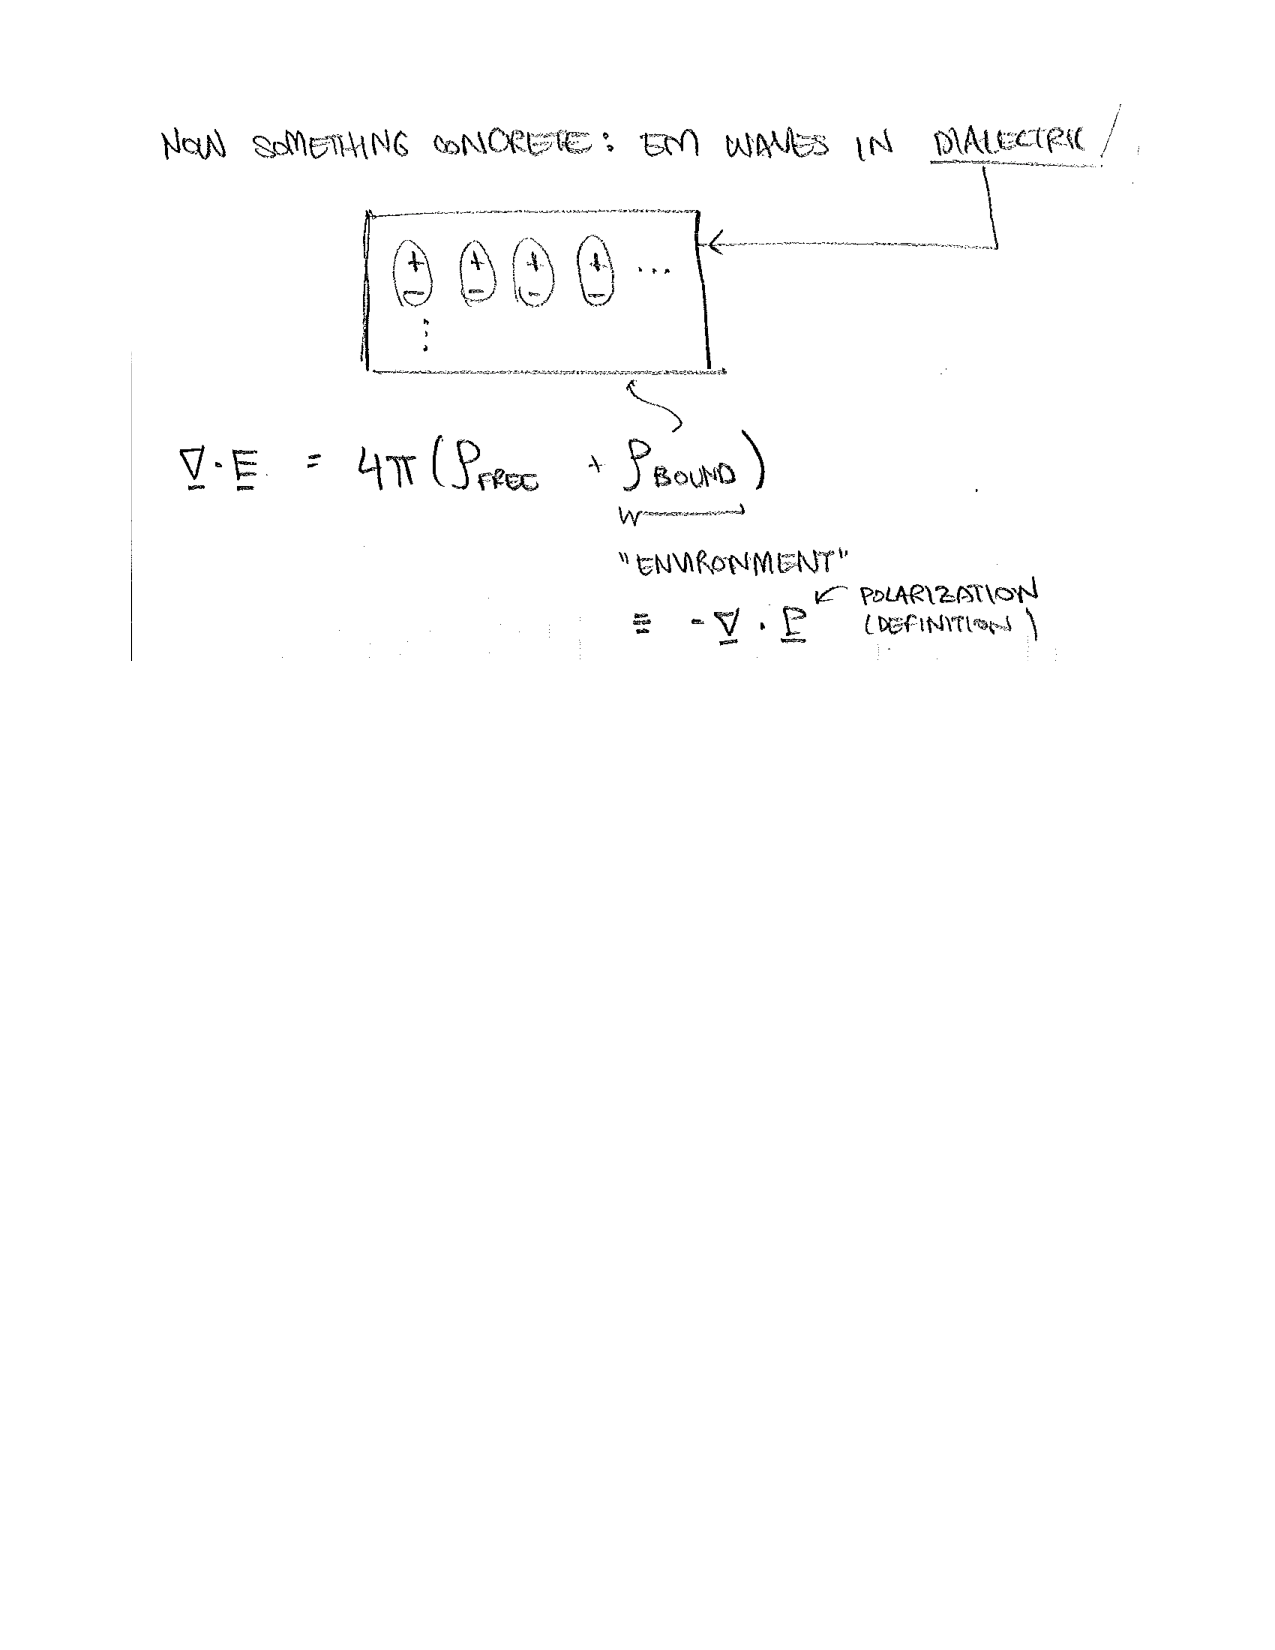
\includegraphics[width=.7\textwidth]{figures/Kramers_01.pdf}
\end{center}

We can split the charge density $\rho$ into free charges and bound charges so that the relevant Maxwell equation is:
\begin{align}
	\nabla \cdot \vec{E} &= 4\pi (\rho_\text{free} + \rho_\text{bound}) \ .
\end{align}
In turn, we may define the \textbf{polarization}, $\vec{P}$, with respect to the bound charge as the electric field sourced by the charge:
\begin{align}
	\rho_{\text{bound}} \equiv - \nabla \cdot\vec{P} \ .
\end{align}
This is a \emph{response} field to the initial electric field $\vec E$. Rearranging this gives
\begin{align}
	\nabla \cdot (\vec{E} + 4\pi \vec{P}) = 4\pi \rho_\text{free} \ .
\end{align}
We sometimes identify the dielectric displacement $\vec{D} \equiv \vec{E} + 4\pi \vec{P}$. For electric fields that are not too strong,\footnote{Can you explain on physical principles what `too strong' means? When does this model break down?}, many materials have the polarization parallel to the electric field:\footnote{You should appreciate why this is the `obvious' thing and reflect on what it would take for a material \emph{not} to obey this.}
\begin{align}
	\vec{P} \equiv \chi \vec{E} \ ,
	\label{eq:KK:polarization}
\end{align}
where we have defined the constant of proportionality to be $\chi$, the electric susceptibility. One may define the permittivity $\varepsilon \equiv 1+4\pi\chi$ so that it is the proportionality between the dielectric displacement and the electric field: $\vec{D} = \varepsilon \vec{E}$.

\paragraph{Waves through a medium.} Now let's imagine what happens when an electromagnetic wave passes through the medium. For our purposes, the wave is just a time dependence on the electric field, $\vec{E}(t)$.\footnote{And you should appreciate how much we're sweeping under the rug here.} The key point is that the susceptibility is \emph{frequency-dependent} $\chi(\omega)$. This should be clear to you intuitively: the microphysics of bound charges react to the changing electric field with respect to some characteristic time scale. It is a harmonic oscillator, after all.


In fact, we may write \eqref{eq:KK:polarization} as
\begin{align}
	\vec{P}(\omega) &= \chi(\omega) \vec E(\omega) \ .
	\label{eq:KK:P:XE}
\end{align}
The $\vec{P}(\omega)$, $\chi(\omega)$, and $\vec{E}(\omega)$ written here are the Fourier components of functions of time, $\vec{P}(t)$, $\chi(t)$, and $\vec{E}(t)$. Forgive me for not indicating tildes ($\tilde \chi$), hopefully making the arguments explicit will avoid confusion.


Let's be clear what we're doing: we want to treat the medium as some homogeneous background. In this background, the speed of light happens to be a bit slower: $v < c$. We define the ratio of the speed of light in vacuum to the speed of light in the homogeneous medium, $n = c/v$, the index of refraction. This is related to the microphysics by $n = \sqrt{\varepsilon\mu}$. For a pure dielectric (no magnetic funny business so $\mu=1$ in appropriate units), this is simply $n=\sqrt{\varepsilon} = \sqrt{1+4\pi\chi}$. What we're saying is that we \emph{know} that there's microphysics (bound charge) that does something weird. We also \emph{know} that fundamentally the speed of light is $c=1$. However, dealing with an Avogadro's number of bound charges is a pain. Instead, we realize that we can \emph{model} the complicated system of bound charges with respect to a susceptibility $\chi(\omega)$. This is an example of an effective theory, an idea that underscores everything that we do in physics.\footnote{Remember: we work with models. Good models are reasonable approximations with well defined limits where they are no longer good approximations. Do not confuse the model with nature, which is the complicated system that we're trying to approximate.}

Let's ignore polarization for this discussion. That's not where the key feature is. An electromagnetic wave of some polarization propagates as
\begin{align}
	\vec E(x,t) \sim \vec{E}_0 e^{ikx - i\omega t} \ .
\end{align}
For simplicity we assume a plane wave moving in the $x$ direction so we ignore the $y$ and $z$ dependence. The momentum/wave number $k$ is related to the angular frequency/energy by $k = \omega/v$, where $v$ is the velocity of the wave in units of $c$.
\begin{exercise}
Confirm for yourself that it is `obvious' that $v = \omega/k$ is the wave velocity. You can start with dimensional analysis, then remind yourself what $k$ and $\omega$ mean physically for a propagating wave.
\end{exercise}
Plugging in the susceptibility gives 
\begin{align}
	\vec E(x,t) \sim \vec{E}_0 e^{i\sqrt{1+4\pi \chi}x - i\omega t} \ .
\end{align}
Implicit here is the assumption that $\chi(\omega)$ is a real number. Perhaps it is not. However, it certainly has a real part. $\text{Re}[\chi(\omega)]$ is the \textbf{dispersion} of the medium. It gives the frequency-dependence of the index of refraction $n\sim v^{-1}$. This frequency dependence tells us how prisms and rainbows work according to Snell's law.

If there is an imaginary part, $\text{Im}[\chi(\omega)]$, it corresponds to \textbf{dissipation}. It's a damping of the wave at a given frequency. Writing
\begin{align}
	k = \frac{\omega}{v} = k_R + i \kappa \ ,
\end{align}
we have the expression for a dissipative wave:
\begin{align}
	\vec E(x,t) \sim \vec{E}_0 e^{-\kappa x} e^{ik_Rx - i\omega t} \ .
\end{align}

\paragraph{Kramers--Kr\"onig.} Let us now pull in two observations:
\begin{enumerate}
\item The susceptibility as a function of time, $\chi(t)$, is a Green's function. We can see this because \eqref{eq:KK:P:XE} tells us that $\vec{P}(\omega) = \chi(\omega \vec{E}(\omega))$ and we know from the convolution theorem in Section~\ref{sec:convolution:theorem} that this means $\vec{P}(t) = \int dt' \chi(t-t')\vec{E}(t)$, which is precisely the form of a Green's function solution to the polarization response to an external electric field $\vec{E}$.
\item We may invoke the Kramers--Kr\"onig relations \eqref{eq:KK:Cauchy:relations} to relate the real and imaginary parts of $\chi(\omega)$.
\end{enumerate}
Recall that the Kramers--Kr\"onig relations relate the real part of an analytic function on the real line to a principal value integral of the imaginary part of the function (and vice versa with `real' $\leftrightarrow$ `imaginary'). 

Is the susceptibility analytic? We know that physics is causal. So in the so-called time domain, $\chi(t)\sim \Theta(t)$. That is, $\chi(t<0)=0$. We want the retarded Green's function where the polarization is \emph{caused by} the external field $\vec{E}(t)$. The system may lag in its response to the external field---and indeed, this is the nature of the slower speed of light in the medium---but it may not \emph{anticipate} the electric field. This causality is imposed by an $i\varepsilon$ prescription on the poles of the Fourier integrand, just as we saw for the harmonic oscillator.\footnote{You can stop to think about why the bound charges really are harmonic oscillators.} Causality tells us that the poles are in the lower half plane (perhaps infinitesimally), so that the integral along and above the real line is analytic. Then the Kramers--Kr\"onig relations tell us
\begin{align}
	\text{Re}\left[\chi(\omega)\right]
	&=
	\frac{i}{\pi} \mathcal P \int d\omega' \frac{\text{Im}\left[\chi(\omega)\right]}{\omega'-\omega}
	\\
	\text{Im}\left[\chi(\omega)\right]
	&=
	\frac{-i}{\pi} \mathcal P \int d\omega' \frac{\text{Re}\left[\chi(\omega)\right]}{\omega'-\omega} \ .
\end{align}
Since $k=\sqrt{1+4\pi\chi}$, the real and imaginary parts of $\chi$ determine the dispersion (rainbows) and the dissipation (absorption) of the medium. Evidently, these two properties of a medium are not independent from one another. 

\begin{example}
You may wonder what this is good for. As a theorist, I certainly wonder this. It turns out that measuring the index of refraction is usually challenging. On the other hand, measuring absorption can be simpler: you just measure how much energy comes out of a material compared to how much energy went in. In this way, by measuring the absorption you can measure everything there is to know about the susceptibility of the material.
\end{example}

\begin{example}
This shows up in quantum mechanics and quantum field theory as the optical theorem. By calculating the amplitude for a particle to `fall out' of a particular Hilbert space due to decay into other particles, you also calculate corrections from virtual particles to its propagation. When you see this in quantum mechanics, you may stop a moment to think: ``it's odd that we're taking the imaginary part of this function.'' If you are too quick, you may dismiss this as quantum mechanics being strange because everything is complex. However, if you are cautious, you'll realize that we're really invoking cousins of the Kramers--Kr\"oning relations.
\end{example}

\paragraph{Why this has to be true.} He's a plausibility argument\footnote{Full disclosure: I learned this on \emph{Wikipedia}.} Imagine that you have some medium that you shine a Gaussian wavepacket of light into. By Gaussian I mean you shine a pulse of some duration that has the shape of a bell-curve in $t$:
\begin{center}
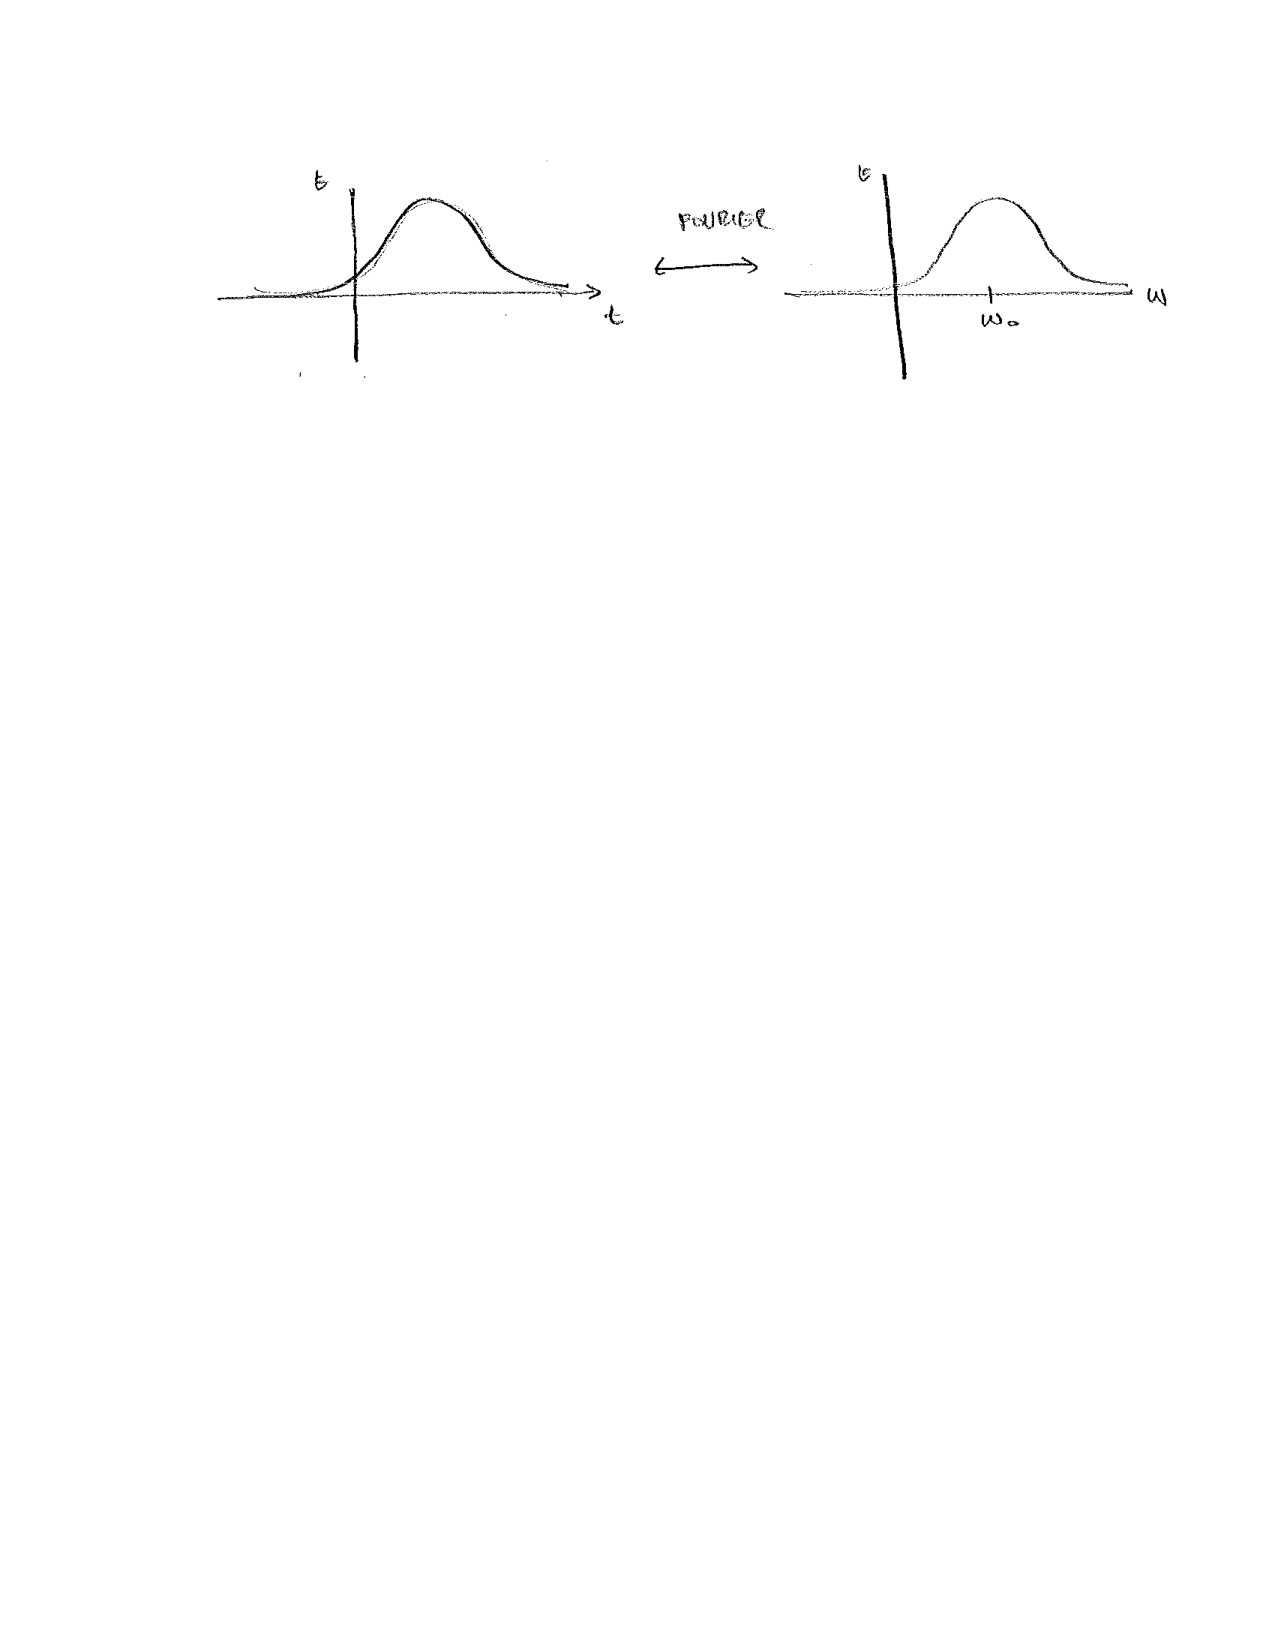
\includegraphics[width=.7\textwidth]{figures/Kramers_02.pdf}
\end{center}
The vertical axis is the field amplitude. As you know, the Fourier transform of a Gaussian is a Gaussian. So the pulse is a Gaussian in frequency space as well. 

Now suppose that this material had a magical property: it \emph{perfectly} absorbs \emph{one} frequency of light: $\omega_\times$. If you want to be realistic you can imagine some tiny-but-finite width around $\omega_\times$. Further, let's assume that there is no dispersion---it's a magical material for which all frequencies of light travel at the same velocity, except frequencies around $\omega_\times$ which do not propagate at all. This means that the electromagnetic wave \emph{after} passing through the material has a $\delta$-function gap in it at $\omega_\times$:
\begin{center}
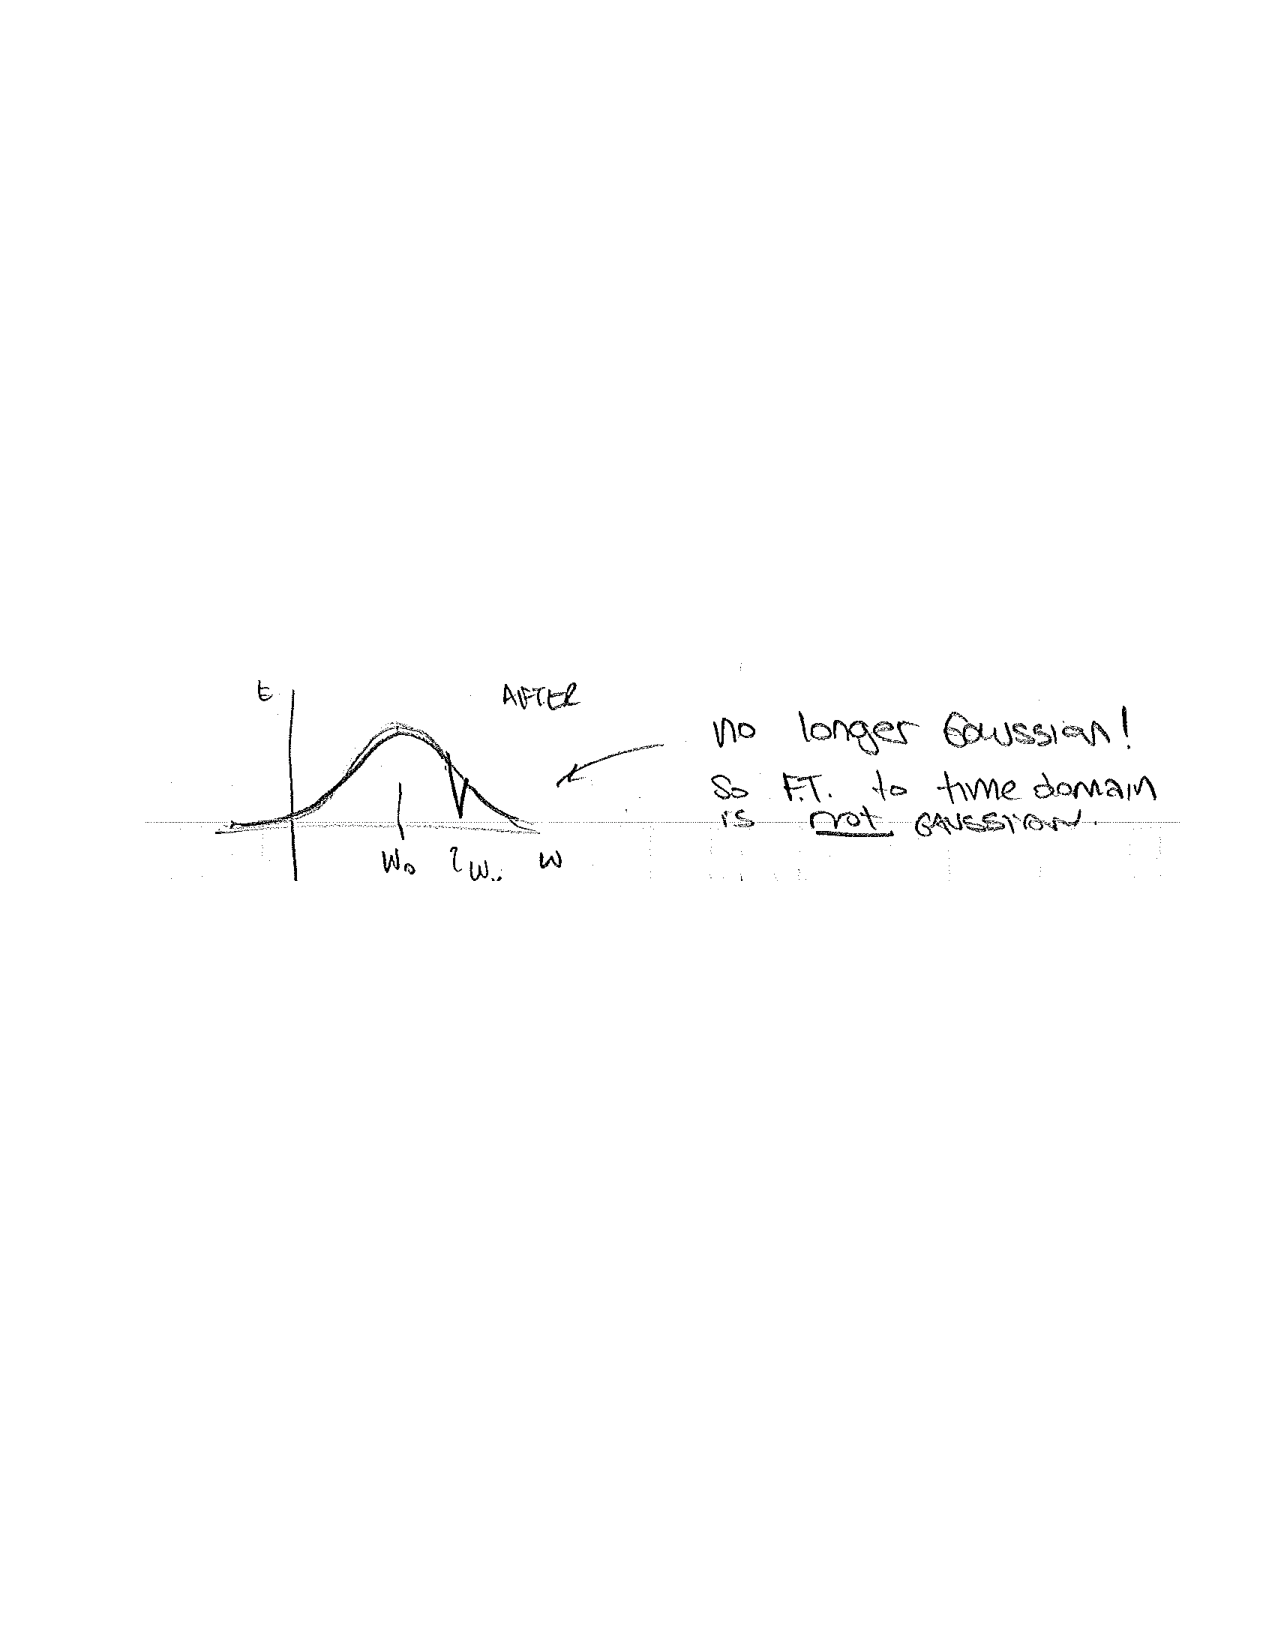
\includegraphics[width=.5\textwidth]{figures/Kramers_03.pdf}
\end{center}
By linearity, we can think about this as a Gaussian plus a $\delta$-function spike:
\begin{center}
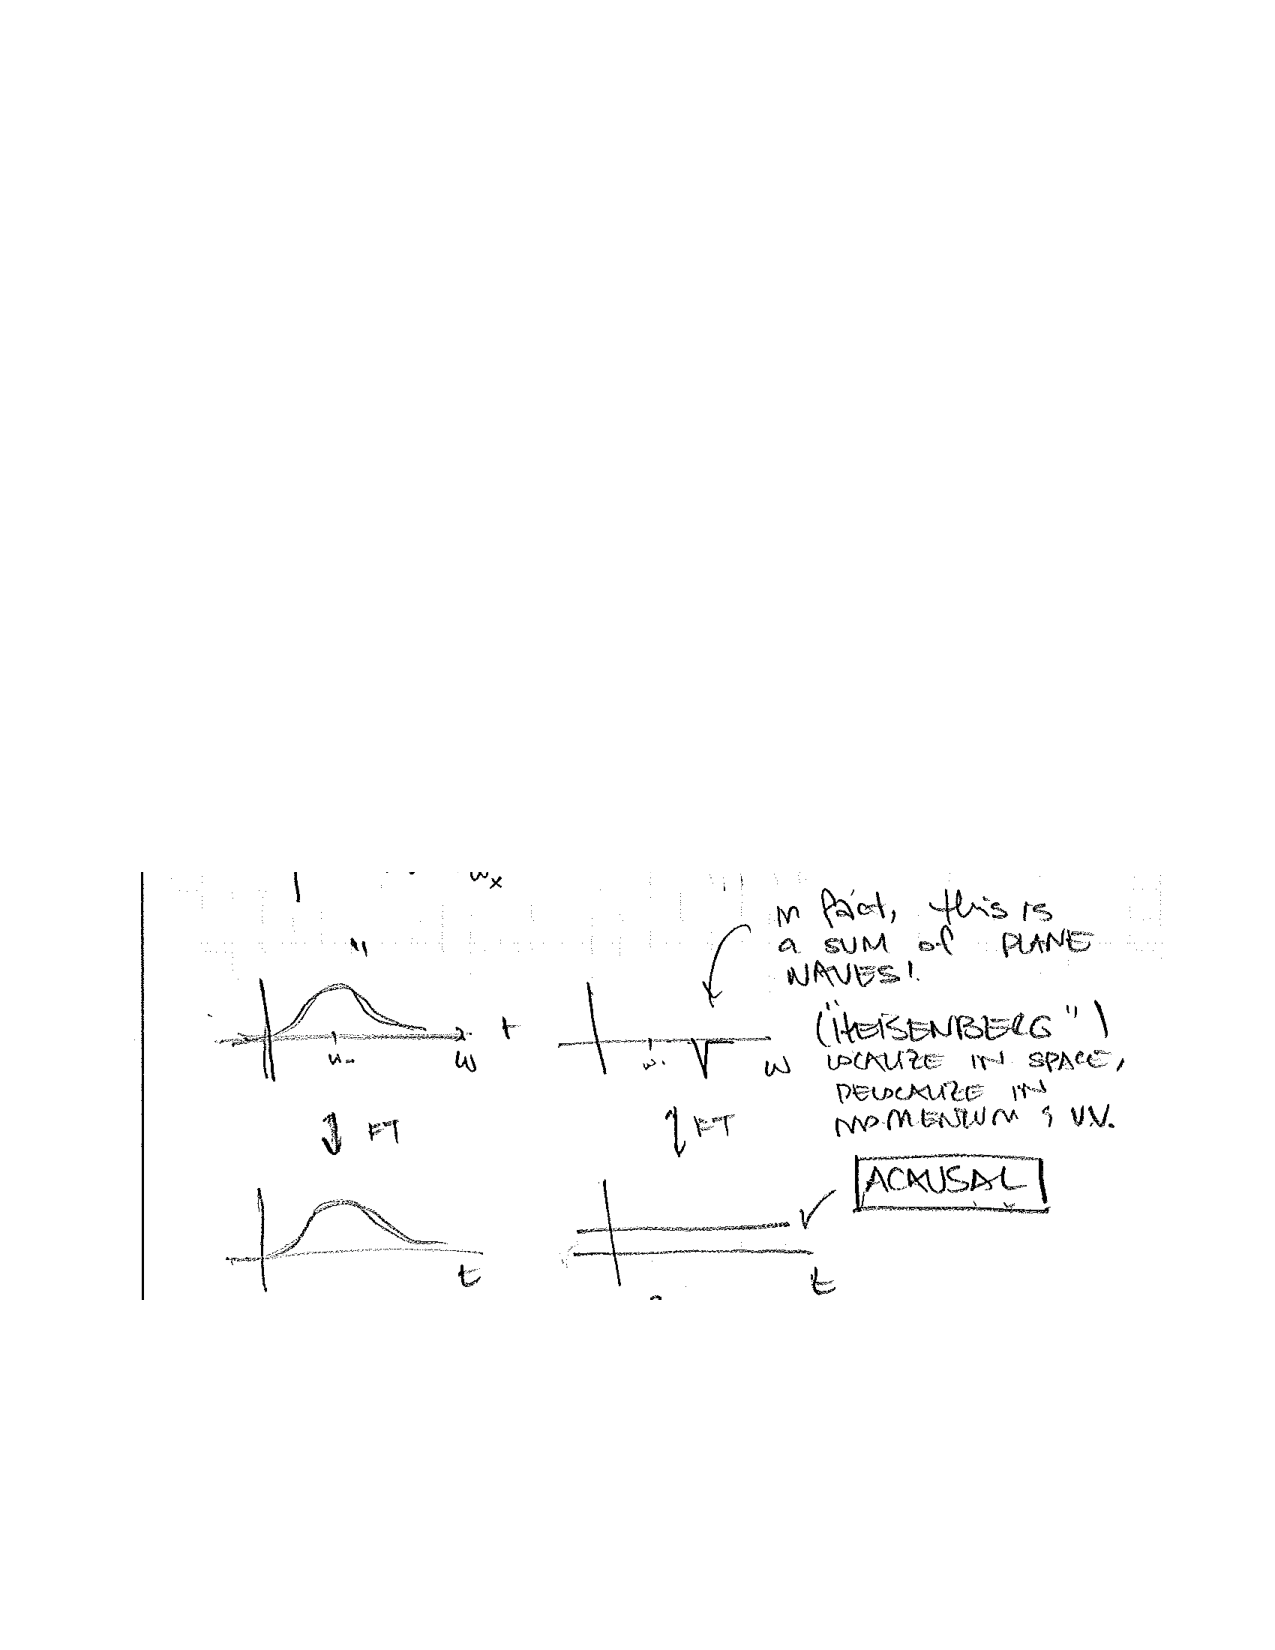
\includegraphics[width=.7\textwidth]{figures/Kramers_04.pdf}
\end{center}

Now we have a problem. The Fourier transform is also linear, so we can Fourier transform each component. The Gaussian in $\omega$ becomes another Gaussian in $t$. However, the $\delta$-function in $\omega$ becomes a \emph{flat distribution} in $t$! Remember Heisenberg's uncertainty relation? This is it: if you localize in one variable, you maximally delocalize in a conjugate variable. This should really bother you: this $-\delta(\omega-\omega_\times)$ spike gives contributions from $t<0$ to $\vec{E}_\text{after}(t)$! What do we make of this apparent paradox?


There is a nice resolution in terms of odd and even parts of $\chi$ with respect to time reversal. Let us define
\begin{align}
	\chi_+ &= \frac{1}{2}\left[\chi(t) + \chi(-t)\right]
	\\
	\chi_- &= \frac{1}{2}\left[\chi(t) - \chi(-t)\right] \ .
\end{align}
You already know that $\chi(t<0)$ is zero, but this separation is instructive since the above analysis seems to be probing $t<0$. Let's go to momentum space with the inverse Fourier transform:
\begin{align}
	\chi(\omega) &= \int dt\,  e^{i\omega t} \, \chi(t)
	\\
	&=
	\int dt\,  \left[\cos(\omega t)+i\sin(\omega t)\right] 
	\, \frac{1}{2}\left[\chi_+(t)+ \chi_-(t)\right] \ .
\end{align}
Now use the fact that the integral over all space of an odd times an even function vanishes. This means that the $\cos(\omega t)$ term only has non-zero integral when multiplying the $\chi_+(t)$ term, and similarly with $\sin(\omega t)$ with $\chi_-(t)$. Thus
\begin{align}
	\chi(\omega) &= 
	\frac{1}{2}\int dt\, 
	\cos(\omega t) \chi_+
	+
	\frac{i}{2}\int dt\, 
	\sin(\omega t) \chi_-
	\equiv
	\text{Re}[\chi(\omega)]
	+i
	\text{Im}[\chi(\omega)] \ ,
\end{align}
where we have explicitly identified the real and imaginary parts. That is to say: the real part is the piece that is \emph{even} in time and the odd part is the piece that is \emph{odd} in time. Both the even and odd pieces give acausal propagation, but when combined in equal parts, you have only causal propagation. The Kramers--Kr\"onig relation enforces causal propagation.

There's an excellent graphic from Wikipedia\footnote{``Kramers--Kronig relations,'' image by user FDominec, \acro{CC BY-SA 3.0}.}:
\begin{center}
\includegraphics[width=.9\textwidth]{figures/Kramers_05_Fdominec.pdf}
\end{center}
What we see in this figure is that the relation between the real and imaginary parts of $\chi(t)$ are precisely what forces $\chi(t<0) = 0$. In frequency space, one cannot simply posit that one frequency is absorbed without any implication on the dispersion of other frequencies. This would violate causality. The resolution to our paradox is that we cannot have a magical material that only absorbs in one frequency \emph{without} causing dispersion. We had stated this assumption with the [wrong] understanding that dispersion and disspation are independent properties that we can tune with microphysics. Evidently, one cannot construct a material whose polarizability is `stiff' to only one frequency without introducing a frequency-dependence to the speed of light across other frequencies.


\flip{In Progress. To do: fourier transform of Theta function.}



